\chapter{Background}
In this chapter, we are going to prepare the reader with basic foundations to understand the work implemented by this thesis.
We are going to focus on the design of the LLVM compiler framework, its IR and its subproject, MLIR.
LLVM COMPILER TOOLCHAIN
(DIFFRENT STEPS AND PASSES AND ESPECIALLY CODE GENERATION)
THEN LLVM IR
THEN MLIR 
RISC-V
SEMANTICS AKA HOW THEY ARE DISPLAYED NOWDAYS
    LLVM IR SEMANTICS 
    RISCVV SEMANTIC (SAIL)

LEAN4 THEOREM PROVER 
    BASICS
    PROVING IN LEAN
    BV DECIDE AND LEANS BIT VECTOR LIBRARY

LEAN-MLIR FRAMEWORK (INTRODUCE IT VERY SIMPPLE AND GO IN MORE EPTH LATER )

\subchapter{The LLVM compiler ecosystem}
The LLVM project is an open-source collection of modular and reusable compiler components and toolchain technologies. It was started as a research project and gained in popularity such that it now is used as the compiler framework various programming languages. In this section we will the explain the compilation flow of LLVM and familiirze the reader with the its IR and the MLIR project within LLVM.

\subsubsection{LLVM compiler design}
Compilers are tools that translate a source program written in a high-level language into their machine code representation. Traditionally, compiler based on the LLVM project compromise the following stages:
\begin{enumerate}
  \item Lexing: Source code gets transformed into a token stream.
  \item Parsing: Converts the token stream into an abstract syntax tree (AST).
  \item Emit IR: AST to IR.
  \item IR-to-IR optimizations
  \item Code generation: IR to machine code lowering.
\end{enumerate}
LLVM itself is not a full compiler, but it provides the infrastructure for the last two stages of compilation stage. After providing a frontend that lowers to LLVM IR, any source langauge can leverage the optimization tools and code generation provided by LLVM. 

LLVM exhibtis its own intermediate representation which is used throught the entire LLVM toolchain. LLVM IR abstracts away source language specic features that would not allows to optimize in


LVM IR focuses on providing a language that is less abstract than a fully source level language but allows for enough of abstraction to employ optimizations that apply across various machine targets, unlikely assembley level optimizations.
a plattform indpenednt way but is still more high-level then assembly code where a lot of the semantics for opitmizations is hidden. 
LLVM IR is optimized in an iterative manner by applying diffrent analysis and optimization passes to its IR in an modular way. These passes are assumed to preserve code integrity and the semantics of the original source program. A pass within LLVM's transformation pass list is InstCombine,which applies peephole rewrites to programs in their LLVM IR form. A user can define which pass to apply by providing the corresponding flag to the LLVM optimizer via the command line or use the predefined set of optimization passes by LLVM by providing the optimization flags -01 to -O3.
Many programming langages provide a front-end, which compiles source code to LLVM IR and then leverages the LLVM backends.
LLVM code generator consists of three substages:
[insert code generation: legalization -> instruction selection -> instruction scheduling].
The modular design of LLVM allows the backend to be reused for any source language that compiles to the specific target architecture.


\textbf{LLVM and LLVM IR}
LLVM IR is a target-independent intermediate representation (IR) at the core of the LLVM (Low-Level Virtual Machine) compiler framework. LLVM is a open-source compiler infrastructure used in academia and industry. LLVM compilers typically lower source programs from high-level languages such as C, C++, Rust, or Haskell into LLVM IR. This intermediate form serves as a common, platform-independent abstraction over machine code to which source languages get lowered before  machine code is omited. Therefore LLVM IR acts as the central language throughout the LLVM compilation pipeline. Once a program is lowered into LLVM IR, a series of IR-to-IR transformations are applied. After these transformations, various LLVM backends further lower the optimized IR into machine code for a specific target architecture. By decoupling the optimization and backend phases from the source language, LLVM IR facilitates reuse and simplifies backend development. LLVM IR focuses on providing a language that is less abstract than a fully source level language but allows for enough of abstraction to employ optimizations that apply across various machine targets, unlikely assembley level optimizations. This abstraction makes LLVM IR suitable for implementing optimizations that are shared and reused across different source and target languages. Thus the implementation and verification of LLVM components, as well as components that interface with LLVM IR can be reused across a wide range of source languages that target LLVM.
\begin{figure}[htbp]
  \centering
  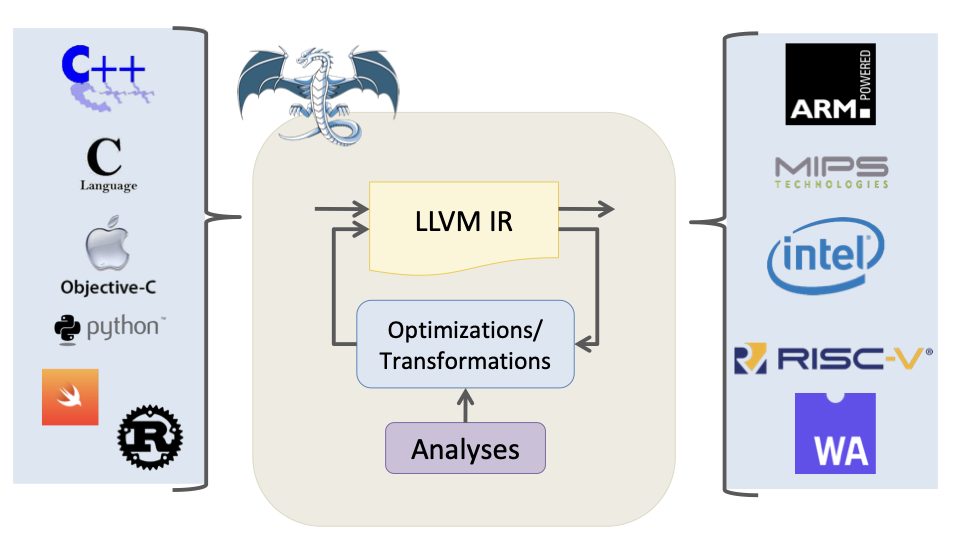
\includegraphics[scale=0.37]{thesis/llvm.png}
 
  \caption{LLVM compiler infrastrucutre with LLVM IR at its heart}
  \label{fig:your-label}
\end{figure}

LLVM IR is typed and in single static assignment form (SSA), which means that every variable has a type and is associated with only one specific definition point in the code. This allows for simplified compiler optimizations along def-use chains, as any use of a variable can be backtracked to a single place where the variable receives a value (def). 

[TO DO INSERT OVERVIEW OF LLVM IR ]

LLVM IR supports common types such as integers of different widths, as well as structured data. To handle non-initialized variables, LLVM IR supports an undef constant in its IR, which represents a set of possible values. When the LLVM compiler encounters an undef it is free to pick any convenient value of the correct type. Besides undef, LLVM IR  has poison values and undefined behaviour. All of these different notions of the future, where the compiler does not want to provide guarantees for a specific value or indicates a unsafe operation. This in turn makes the semantics of LLVM IR inherently non-deterministic and will be discussed in detail in section []. 